\documentclass[12pt]{report}

% These are necessary to compile
\usepackage{graphicx}
\usepackage{hyperref}
\usepackage{amsmath}

% Don't know which ones of these we actually use
%%\usepackage{setspace}
\usepackage{amsfonts}
\usepackage{amssymb}
\usepackage{amsthm}
\usepackage{enumerate}
\usepackage{mathrsfs}
\usepackage{alltt}
\usepackage{color}
\usepackage{chngpage}
\usepackage{fancyvrb}
\usepackage{epstopdf}
\usepackage{url}
\usepackage{verbatim}
%\usepackage[autostyle]{csquotes}
%\usepackage[toc,page]{appendix}

% Setting the page alignment with this package
\usepackage[top=1in, bottom=1.5in, left=1.5in,right=1.5in]{geometry}

\DeclareGraphicsExtensions{.png}

\hypersetup{
    colorlinks=true, %set true if you want colored links
    linktoc=all,     %set to all if you want both sections and subsections linked
    linkcolor=black,  %choose some color if you want links to stand out
    citecolor=black
}

\hyphenation{MTA SZTAKI}

\begin{document}

% TODO make title page look nicer
\begin{titlepage}
\begin{center}
\thispagestyle{empty}
% TODO install \textsc font
\Large{\textbf{A Major Qualifying Project Report\\ \large{ON}}}\\[1.75cm]
\LARGE{\textsc {\textbf{Improving the Speed of Peer to Peer Backup Systems with BitTorrent}}}\\[0.5cm]
\vspace{0.25cm}
\Large{\textbf{\\Submitted to the Faculty of }}
\LARGE{\textbf{\\WORCESTER POLYTECHNIC INSTITUTE\\}}
\vspace{0.5cm}
\Large{\textbf{\\In Partial Fulfillment of the Requirement for the}}
\Large{\textbf{\\Degree of Bachelor of Science}}
\vspace{0.5cm}
\Large{\textbf{\\by}}\\[0.75cm]
\large{\textbf{Dan Bouffard}}\\
\large{\textbf{Marc Green}}\\
\vspace{0.75cm}
\large{\textbf{UNDER THE GUIDANCE OF}}\\
\large{\textbf{Professor G\'abor N. S\'ark\"ozy}}\\
\vspace{1.5cm}
\large{\textbf{\\May 1, 2014}}\\
\end{center}
\end{titlepage}

\begin{abstract}
For many computer users, having access to a reliable file backup service is important. As computers and computer-related technologies improve, users have the ability to generate higher resolution content. Creating backups becomes less feasible as the amount of data grows; limited network bandwidth makes the backup process cumbersome, and access to a large amount of storage space for backups is either limited or expensive. In this report, we propose a new backup system, BTBackup, which aims to solve both problems. Our system is designed as a Peer-to-Peer (P2P) network, where users of the system use each other as backup locations. Users offer storage space that is proportional to the amount of data that they backup. This means that the capacity of each user's physical storage is the only limiting factor for how much they can back up. We solve the problem of long data transfers for big files by leveraging the speed offered by the BitTorrent Protocol, which uses a file chunking mechanism to download files from multiple peers at once. By testing our system in various scenarios, we show that it achieves our goal of quicker backup creation through the use of file transfer parallelization.
\end{abstract}

\renewcommand{\abstractname}{Acknowledgements}
\begin{abstract}
% TODO adjectives
% TODO format this section better
Mih\'aly H\'eder, our on-site Project Advisor, for his advice, insight, expertise, and bottomless teapot.\\

\noindent G\'abor S\'ark\"ozy, our off-site Project Advisor, for his guidance, encouragement, and editorial skills. \\

\noindent Worcester Polytechnic Institute, for the opportunity to study abroad. \\

\noindent MTA SZTAKI, for the resources to design, develop, and test our system. \\

\noindent The employees of MTA SZTAKI, for their open arms and continued friendship.
\end{abstract}

\tableofcontents
\listoffigures

% TODO: Talk about how fast transfer are important for P2P backup in particular, since many replicas will need to be made and replicas will need to be moved around.
\chapter{Introduction}

As the capacity and performance of hard drives continue to increase over time, users continue to store their data in greater volumes. This includes high resolution photos, videos, and audio for the personal user, and databases, source code repositories, and operating system images for the technical user. The increase in stored data gives rise to a greater need for the data to be backed up, in preparation for the undesirable event that one's hard drive becomes inaccessible. This can happen if one's computer crashes, the hard drive fails, or the computer is lost or stolen.

Most backup systems that are in use today are centralized, meaning that they rely on some central entity to store their data. This entity is typically a company that offers data backup as a service, such as Dropbox or Google. While these solutions are somewhat convenient, since the service is guaranteed to almost always be online, there are several problems with this approach. The amount of data that users can backup is severely limited, and obtaining more space costs money. In a time where owning terabytes of data is common, cloud storage meant for everyday use is not a feasible backup solution. Dedicated backup solutions can offer an adequate amount of space, but often require expensive recurring payments for their service. In addition to this, users must trust the entity to which they send their data to both remain online and respect their privacy. This trust is not always possible.

Although they have not gained much popularity, peer to peer (P2P) file backup systems have been created and studied by researchers for over a decade. These systems do not suffer from the aforementioned drawbacks of centralized systems; they are free to use, limited in storage only by the user, and do not require a trusted central entity. Instead of backing up their data to a server, peers back up their data to \textit{each other}. However, abandoning the centralized server model in favor of a distributed one brings with it new problems that must be addressed before wide-spread adoption can be expected. Research in this area has focused on topics such as handling node churn\footnote{Node churn refers to the continuous arrival and departure of nodes in a P2P network. See Sections  \ref{subsec:PeertoPeerNetworks} and \ref{sec:churn} for more detail.} \cite{ChurnResilient}, efficient routing algorithms \cite{Kademlia}, and minimizing bandwidth \cite{PeerStore}.

We have designed and implemented a new P2P backup system, called \mbox{BTBackup}, that improves the speed of backing up and recovering data. Our primary contribution, and the technology responsible for faster file backup and recovery, is the way in which we handle data transfer: BitTorrent Sync, a new synchronization application created by BitTorrent, Inc. BitTorrent Sync uses a modified version of the BitTorrent protocol \cite{BTSyncFAQ} in order to quickly synchronize files between groups of peers. This protocol is especially effective at transferring large files, which makes its use perfect for the domain of P2P file backup. By leveraging BitTorrent Sync, we take advantage of BitTorrent's ability to better utilize a peer's bandwidth by downloading from multiple sources at once. This is in contrast to other P2P backup systems, which directly download from one source at a time. Our approach takes advantage of the fact that P2P backup systems require data replication, the act of inserting several redundant copies of data into the network, to combat node churn. We view the set of nodes storing replications for a given file as a BitTorrent swarm, allowing us to use the BitTorrent protocol without additional overhead.

A secondary contribution of our research is the testing infrastructure we have designed. We created test scenarios to (1) measure the extent to which BitTorrent increases data backup and recovery transfer speeds, and (2) ensure our system is a feasible backup solution under realistic conditions. To test the former, we measured the rates of data transfer over time when backing up 1 GB of data. In order to see the effects filesize has on speed, we ran this test thrice: once with one 1GB file, once with ten 100MB files, and once with one hundred 10MB files. To test the latter, we created a test scenario that simulated usage of our system in a realistic environment. Each instance of this scenario created 100 peers on a network using MTA SZTAKI's cloud computing environment: SZTAKI Cloud. Specifically, this scenario measured the effects of node churn, or the rate at which nodes enter and leave the network, on our system. Since our system handles churn by moving replicas from unavailable nodes to available ones, we measure how much extra network traffic is generated to see the effects of churn. We take this measurement by running a test instance with no churn, and then running another one with churn. To provide a realistic setting, we had each peer limit their download and upload speeds to values that are based off of worldwide Internet bandwidth statistics.

After running our tests, we found that BitTorrent performs well as the data layer transport protocol for a P2P backup system. Specifically, we found that \emph{larger but fewer files are handled more efficiently than a greater number of smaller files}, given the same amount of total data. We also determined that our system handles node churn well, when the rate of churn is modeled off of the average Internet user. Our final and most important result is that \emph{our system was able to achieve data transfer rates up to \~300\% quicker than the rates that could be realistically achieved in traditional backup systems.}
% TODO emphasize that our system handles node churn well, but need to reword/give numeric data
% TODO add (first, create) result of file backup speed increase percentage

The rest of this paper is organized as follows. Chapter \ref{chap:Background} introduces the reader to the concepts and ideas necessary to understand our system, including glimpses into other peer to peer systems. Chapter \ref{chap:BTBackup} describes the design of our system; Chapter \ref{chap:impl} describes our implementation of it. In Chapter \ref{chap:Methodology}, we discuss how we tested our system, and Chapter \ref{chap:Results} analyzes the results. Finally, Chapter \ref{chap:Conclusion} concludes our paper and outlines future work to be done.

\chapter{Background} \label{chap:Background}
\section{Centralized Backup Systems}
Several popular backup systems currently in use have a centralized system design. In these systems, there are many clients that all back up their data to a central location controlled by a single entity. Common elements of these systems include a fixed amount of data storage per person, with the option to obtain more for a fee. Three of the more popular systems are Google Drive, Dropbox, which has over 200 million users \cite{dropboxusers}, and OneDrive, with over 250 million users \cite{onedriveusers}.

There are several benefits to using a centralized backup system. The first is that it is very probable that the service will always be on, as the content is being stored on servers dedicated to that purpose. Companies who offer file backup services have the hardware resources to store redundant copies of data, should a server fail. They will also have the personnel to investigate and fix any problems with the service.

However, there are also several problems with using a centralized system to back up data. One of these problems is that there is a single point of failure, should the storage site be compromised in some way (for example, natural disasters). This is less of a problem for big companies with the resources to handle these situations, but there is still a cost to take the necessary preventative measures when creating the system.

Another problem with centralized systems is a matter of trust: when a user stores his or her data using a third party, the third party essentially has control of that data. Even if the third party claims to offer encryption for all data that they hold, there could still be a backdoor in the service that allows them or another entity to obtain an unencrypted version of the data. One solution to help combat this is to manually encrypt the data before sending it to the third party, but this is hardly a convenient solution.

Finally, there are often restrictions on what can be stored using centralized backup systems. This includes both the size of individual files and the amount of total data. More space is gained by paying a monthly or yearly fee, but even then the amount of space is capped at a specific size. For users who need to back up a large amount of large files, these systems are not very useful.

Peer to peer backup systems, on the other hand, provide an equivalent service and suffer from none of these drawbacks.

\section{Peer to Peer Backup Systems}

Peer to Peer (P2P) Backup Systems are applications that allow users to back up data without the use of a central entity. Instead, each user offers some of his or her storage space in order to use the space of others as backup locations. We start this section by introducing peer to peer networks, and then discuss the technical components of existing P2P backup systems.

\subsection{Peer to Peer Networks} \label{subsec:PeertoPeerNetworks}

A peer to peer network is a type of distributed network model in which participants form direct connections to each other. This is in contrast to the centralized client-server network model, in which all participating clients connect to a central server to carry out their task. Client-server network models are used on the World Wide Web: the clients are users' web browsers and the server is the website being visited. In peer to peer networks, each participant, or "peer", functions as both a client and a server; peers initiating a request take on the role of the client, and peers answering the request take on the role of the server.

In the client-server model, servers are expected to always be available and accessible. Peer to peer networks do not have this luxury. Instead, they experience the constant fluctuation of peers joining and leaving the network. This is called \textit{churn} \cite{StorageSearchP2PNetworks}. Churn in P2P networks complicates the communication between peers because the sought peer may be offline. This is especially a problem in P2P backup systems; for example, a peer might try to recover data from another peer who is not online. The strategies for dealing with churn, and many other P2P-specific complications, heavily depend on the type of overlay network a P2P application uses. We discuss churn in more detail in Section \ref{sec:churn}.

\subsubsection{Overlay Networks}

An overlay network is any network built on top of another network. That is, an overlay network consists of nodes with neighbors who are not physically connected, but instead use the underlying network to establish a virtual connection. They need not be constrained by the limitations of the physical world. Consider a trivial example where there are three computers connected to the Internet, but located in different parts of the world. These three computers could form an overlay network by agreeing to be virtual neighbors to each other. If their overlay network was used in a P2P application, then, when connecting to each other, they will use the underlying network, the Internet, to actually send messages. The P2P application does not need to know about the underlying network that is used to route messages; it only needs to know that there is an overlay network that defines the direct connections between peers.

Peer to peer applications use overlay networks as their foundation.\footnote{Overlay networks are used for many purposes, not just P2P applications. Note, however, in discussing overlay networks, we will still refer to their participants as \textit{peers}.}  The P2P overlay network provides structure for the application that uses it, allowing peers to find each other.

There are three categories of overlay networks that can be used as the network abstraction on which a P2P network is built. \textit{Structured} overlay networks organize peers according to some geometry, e.g., a ring. This structure is strictly maintained as nodes join and leave the network. \textit{Unstructured} overlay networks, on the other hand, do not organize peers, but instead allow the network to grow into any shape, determined only by the routing table of each peer. \textit{Hierarchical} overlay networks are composed of multiple groups of peers each forming their own overlay network. A representative peer from each group joins a top-level overlay network, connecting the distinct groups \cite{p2pSurvey}.

We discuss structured overlay networks in more detail below, as that is the type of overlay network our P2P backup system uses.

\subsubsection{Structured Overlay Networks} \label{subsubsec:StructuredOverlayNetworks}

Structured overlay networks are defined by a topology and a virtual address space. For example, in our system, peers are organized in a ring and addressed by 20 byte numbers---our address space is the set of all 20 byte numbers. In other systems, peers could be organized in a 3D cube and addressed by their (x,y,z) coordinates. The topology defines the set of neighbors each peer has in the overlay. The address space serves as a way to uniquely identify peers.
% TODO maybe insert figure of chord ring topology (or our own!)

The purpose of peer to peer networks (and more broadly, networks in general) is to share data. In the P2P networks that focus not just on sharing data, but also storing, locating, and possibly retrieving data (like ours), the data shares the same virtual address space as the peers. That is, these structured overlay networks give the data themselves valid addresses. For example, in our system, the data being backed up is also given a 20 byte "address". This is done to determine which peer is responsible for a given piece of data. Specifically, a peer is responsible for all data in the address space that the peer is closest to. It is for this reason that peer address assignment should be evenly distributed, to keep the distribution of work equal.\footnote{The average size of the address space for which a peer is responsible decreases as more peers join the network, which allows these types of networks to easily scale in size.}

To join a structured overlay network, a peer must know at least one other peer already in the network. This peer is often called the \textit{bootstrap peer}. The joining peer will contact the bootstrap peer to find its proper place in the topology. We come back to this below in more detail in our explanation of how to find other peers.

% TODO cite router.bittorrent.com as well known bootstrap node?
%In BitTorrent's structured overlay network \footnote{To clarify, we are referring to BitTorrent's distributed hash table, not its unstructured network. The latter involves using centralized trackers, the former removes such dependency. We refrain from using the term \textit{distributed hash table} to keep the explanation simple without loss of generality. We discuss distributed hash tables in section \ref{sec:backgroundDHT}.}, a well known bootstrap node \footnote{The BitTorrent specification uses \textit{node} to refer to participants of its structured overlay network and \textit{peer} as a more general term \cite{bittorrentDHT}. We will adopt this convention when speaking about BitTorrent, and use them interchangeably otherwise.} is router.bittorrent.com. A BitTorrent node randomly chooses a 160 bit \textit{nodeID} to use as an address. To join the network, it will contact a bootstrap node to find the nodes it is closest to in the topology. Closeness, in BitTorrent's case, is determined by taking the $XOR$ of \textit{nodeID}s; smaller values are defined as closer \cite{bittorrentDHT}.
% TODO define XOR?
% TODO maybe remove this entire paragraph, since it doesn't really clarify anything. it just gives another example of picking an id and mysteriously finding nodes its closest to. if we end up remove it, we should reword end of previous paragraph
% TODO maybe keep it in b/c we refer to closeness in 3.1.1

Leaving a structured overlay network can be as simple as not responding to any messages. Our system, like many others, leaves this functionality undefined. Node failures due to hard shutdowns will not follow the protocol to leave the network, so it is easiest to treat all node departures as node failures.

To find other peers, a peer in a structured overlay network will consult its routing table. This table is initially populated upon joining the network, and is kept up to date as peers join and leave. When a joining peer first contacts a bootstrap peer, it is unlikely that the bootstrap peer has the joining peer's direct neighbors in its routing table. This is because the routing table is designed to include many peers that are close, and only a few peers that are far. A joining peer, by asking the bootstrap node, will learn of the peers in the bootstrap peer's routing table that the joining node is close to. The joining peer will then contact these peers, ask for the same information, and learn of peers it is even closer to. This process repeats until the joining node learns its direct neighbors \cite{p2pSurvey}.

Overlay networks are the abstraction that connects all the users of a P2P system. It is the foundation on which a P2P application can be built, and is responsible for providing methods for peers to join and leave the network, and find other peers in the network. Furthermore, structured overlay networks allow the P2P application to locate specific information very quickly because their virtual address space provides full accountability of any piece of data. It is for this reason we chose a structured overlay network as the substrate of our P2P application; it is easy to determine which peer is responsible for a given backup because we know it will be the one closest in the address space.\footnote{However, churn complicates this. For example, a peer with an even closer address may join the network between storing and retrieving the data.}

% TODO may need better segue between p2p networks and file chunking

% TODO: Ask Sarkozy/Mihaly if they think keeping this section in is worth it.
\subsection{File Chunking} \label{sec:filechunking}
The format in which files are stored can have an effect on the efficiency of the P2P backup system. At first, backing up each file as a whole might seem like the obvious choice, since files are only useful in their entirety. However, the creators of the P2P backup systems pStore \cite{pStore} and PeerStore \cite{PeerStore} have shown that there are benefits to splitting files up into fixed-sized chunks, rather than distributing complete files to peers. In these systems, this is accomplished by creating two types of files: a "file block", which contains a section (chunk) of the original file, and a "file block list", which contains information on which file blocks compose the original file and how to order them. This allows for peer heterogeneity in terms of storage capacity. For example, if a peer needs to store a 10GB file, it does not need to find an individual peer capable of storing 10GB (which might be rare); rather, it needs to find a number of peers, each capable of storing the size of a chunk (which is magnitudes smaller in size than the original file).

Equation \ref{equ:file_chunk_peers} shows how many peers are needed to store a file $F$ for a given chunk size $c$, the number of desired replications of the file $r$, and the size of the file $F_{size}$.

\begin{equation} \label{equ:file_chunk_peers}
\text{Number of peers} = \frac{F_{size}}{c} \times r
\end{equation}

Although lowering the chunk size will increase the chances of finding a peer to store on, it is important to choose a reasonable chunk size, as using more nodes for storage will add more overhead in finding those nodes.

File chunking also gives the benefit of easy versioning and updating of files. When a newer version of a file is backed up, the only chunks that need to be reinserted into the network are the ones that differ from the previous version. Old versions of file chunks stay in the network, so that any full version of the file can be reconstructed by requesting the appropriate file chunks. Backup systems can also reduce the amount of storage space used by sharing identical file chunks between peers.

Our system does not use file chunking. Instead, by using BitTorrent as the data transport protocol, we have applied the concept of splitting files into chunks in a new way in P2P backup systems. We distribute complete files to each backup location, but separate files into chunks when they are being transferred; this is how BitTorrent works. With the BitTorrent Protocol, a peer can download a file by requesting chunks of it from many peers at the same time. By utilizing the upload bandwidth of several peers, a file can be downloaded quicker than if it were directly downloaded from one entity (see Section \ref{sec:TheBitTorrentProtocol} for more details).

\subsection{Fairness} \label{sec:BackgroundFairness}
Another aspect of P2P backup systems is fairness between peers. Peers need to be storing an amount of data proportional to the amount that they are backing up to other peers. This can be challenging to enforce, because untrustworthy peers can attempt to game the system to obtain free backup storage. For example, consider a simple system where each peer must offer to store the same amount of data that they back up on other peers. A peer could claim that all of the storage space that it should be offering is being used by other peers, while in reality the peer has not taken in any other peer's data. It is clear that a mechanism needs to be built into the system that ensures that peers store the data of each other.

PeerStore handles this via a combined trading and challenge system. When a peer wants to create a backup of its data, it finds a peer to trade data with. In its request to back up data, the peer will also advertise that it is willing to store a certain amount of data for its trading partner. The peer that receives the request will then need to accept or reject it, and if the request is accepted, the acceptor will also need to request a certain amount of storage in return. If the original requestor accepts this offer, then the two become trading partners and will send each other data. This process is illustrated in Figure \ref{fig:peerStoreTrading} \cite{PeerStore}.

\begin{figure}
  \centering
  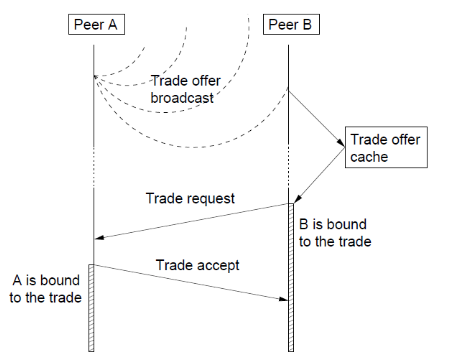
\includegraphics[scale=0.75]{figures/PeerStoreTrading}
  \caption{Trading protocol of PeerStore \cite{PeerStore} \label{fig:peerStoreTrading}}
\end{figure}

While this ensures that peers will agree to take data in proportion to the amount that they want to back up, it still does not guarantee that peers hold onto that data. For example, a peer could form a trading agreement with another peer, exchange data, and promptly discard the received data. To combat this, peers can periodically challenge each other to prove that they are actually storing data. This is the approach that we, like PeerStore, propose. We provide peers the ability to ask each other to prove they are storing the data that they are supposed to be storing. A peer proves itself by replying with a value that could only be derived if they were, indeed, safekeeping the data. See Section \ref{subsec:ChallengeMechanism_sec:Fairness_chap:BTBackup}
 for more details about our proposed challenge mechanism.

\subsection{Churn and Data Migration} \label{sec:churn}
With each storage node being regular users, it is often the case that nodes can be offline. Recall that churn refers to the fact that peers will continuously enter and leave the P2P network. The designer of a P2P backup system must take this into consideration if the system is to provide reliable access to backed up data. This has been accomplished via data migration \cite{pStore,PeerStore}, where the availability of files is periodically checked and replicas are made when the peers being used for backup are not reliably available. Other data migration algorithms have been designed specifically to work in high churn networks \cite{StorageSearchP2PNetworks}. In this case, data replicas are periodically redistributed to different groups of nodes, which means that newer nodes have a chance to store data. This is beneficial because data stays evenly distributed throughout the overlay network, preventing any single node from being responsible for too much data, regardless of when they joined.\footnote{It is important to note this strategy is designed to work in an unstructured overlay network, not a structured one. Structured networks need not redistribute like this because the evenly distributed address assignment provides the even data distribution.}

The number of replicas to maintain will have an impact on the performance of the system. If the replica count is too low, the probability of recovering the file is lowered. If the replica count is too high, then bandwidth and storage space will be needlessly used; the peers storing replicas do not significantly contribute to the availability of the data, and the peer backing up the data will need to store more data for others as part of the fairness mechanism.

\subsection{Cryptography} \label{sec:crypto}
Cryptography is the study of techniques for secure communication in the presence of third parties \cite{cryptoDef}. It is heavily relied upon in the computer world to protect secrets, verify identities, and ensure data has not been tampered with. Our system uses cryptography to \textit{encrypt} users' data before replicating it to strangers' computers. Encryption is the process of obfuscating text into a state such that it cannot be understood without \textit{decryption}, the reverse process. Secret \textit{keys} are used to parameterize encryption algorithms so that, although the specific process for encryption is public, the message it encrypts remains a secret. In \textit{symmetric-key} encryption, the key used to decrypt is identical to the key used to encrypt. This differs from \textit{public-key} encryption, in which two different, yet mathematically related, keys are used.

Encryption in P2P backup systems is necessary to prevent the peers who are storing backups of data from reading it. A system in which backups were unencrypted would be much less popular with users, because they would lose privacy by using it. The terminology associated with this is \textit{confidentiality}, meaning that data that is supposed to be confidential, remains confidential. Our P2P backup system leverages BitTorrent Sync, which uses the AES encryption algorithm to encrypt backups before replicating them.
 % TODO not sure if we should describe AES here... AES is a \textit{symmetric-key} encryption algorithm, which means the same key is used to both encrypt and decrypt.

\textit{Hashing} is the process of applying a function to some arbitrary-length message, resulting in a fixed sized output, or \textit{hash}. \textit{Cryptographic hash functions} have mathematical-based properties, e.g., \textit{pre-image resistance}, that provide certain guarantees (with high confidence) about the resulting hash. Pre-image resistance refers to hash functions that cannot be \textit{reversed}. That is, given $hash(m) = h$, the hash function is pre-image resistant if an adversary cannot find the input $m$ when given the output $h$. The other required properties of cryptographic hash functions are \textit{second pre-image resistance} and \textit{collision resistance}. A hash function has second pre-image resistance if, given an input $m_1$, it is difficult to find a second input $m_2$ such that $hash(m_2) = hash(m_1)$. This is similar to collision resistance, which mandates it is difficult to find any two inputs that map to the same output.
% TODO find math to put here
% TODO why are we explaining these properties of crypto hash functions? do we even use crypto hash functions?

To strengthen hashing algorithms, a \textit{salt} can be utilized. A salt is essentially a randomly picked string of bytes that is concatenated to data to be hashed. The same hash will be calculated if the same salt is used with the same original data. Using salts is a useful technique in preventing \textit{dictionary attacks}, where an attacker compares a precomputed list of inputs and their hashes with a target hash of some unknown data in an attempt to find out what the unknown data is. Dictionary attacks are common on password hashes, because, upon success, the attacker will discover the password used to generate the password hash. With a salt, however, the precomputed hash for the data will not match. The list of hashes cannot be easily recomputed with the salt, since hashing is designed to be an expensive and lengthy operation.

\textit{Convergent encryption} is a technique used in pStore and PeerStore to ensure confidentiality \cite{pStore, PeerStore}. Convergent encryption involves taking the hash of the unencrypted data, and then using the hash as the symmetric key to encrypt the data. The main benefit of using convergent encryption is that the same data will be encrypted the same way each time, so identical blocks in the network can be shared between peers in their encrypted form, without the need for a complicated key exchange protocol. Convergent encryption is illustrated in Figure \ref{fig:convergent}.

\begin{figure} \label{fig:convergent}
  \centering
  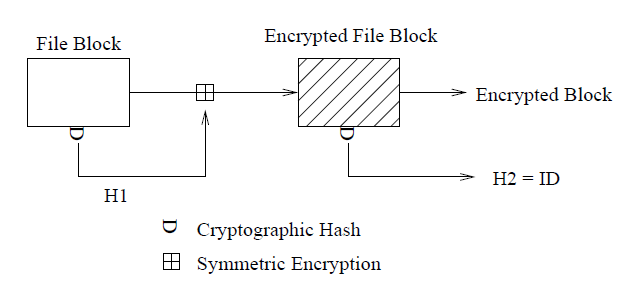
\includegraphics[scale=0.75]{figures/ConvergentEncryption}
  \caption{Convergent Encryption from PeerStore}
\end{figure}

While this is a convenient optimization, it has a security weakness: any user who has access to the unencrypted version of a file can confirm whether or not that file is being stored in the system. This encroaches on users' privacy.

% TODO relate convergent encryption to our system

% TODO digital signatures? discussed in future work

\section{Distributed Hash Tables} \label{sec:backgroundDHT}

A \textit{hash table} is a data structure that maps unique keys to values. It has attractive performance features, such as $O(1)$ average lookup time. This means that, on average, the time it takes to retrieve a value from the hash table is independent of the number of entries being stored. This performance comes from the use of a hash function when organizing the data internally. A hash table can be represented as an array of \textit{buckets}, which are slots used to store the data. Hash functions are used to map a given key to an index in the array of buckets. Thus, given a key, the hash table can compute the bucket in which the (key, value) pair is stored. In the event of hash collisions, the (key, value) pairs in each bucket can be stored as a linked list. Hash tables use hash functions that have uniform hash distribution to minimize collisions, since traversing the linked list is the bottleneck of the operation. Hash tables have $O(1)$ insertion and deletion time for the same reason.

A \textit{distributed hash table} (DHT) is a hash table that is stored across multiple nodes. Each node is responsible for a portion of the hash table's contents. In exchange for distributing the storage cost among several nodes, DHTs do not have $O(1)$ search, insertion, or deletion time. Instead, the $put(k, v)$ and $get(k)$ operations in a DHT are designed such that they can be sent to any participating node. The receiving node will forward it closer to the node responsible for the given key $k$. There is a trade-off between the size of each node's routing table (i.e., who they know about) and how fast operations can be performed.

The cost of routing is acceptable because the usefulness of distributing the storage cost far outweighs the drawback of slower operations on the data structure. The alternative would be to have each peer keep a copy of the entire hash table. This solution suffers from several problems: it makes the hash table hard to maintain, the download time can become nontrivial, and it might become infeasible to store the entire table on regulars peers, since it can become huge with larger networks.

% TODO discuss DHTs being good with churn, scale well

% TODO citations?


DHTs play a major role in many P2P systems. They serve as the means through which peers can find either data or other peers, depending on the system; our system uses a DHT for the latter. In conjunction with the structured overlay network, the DHT allows for peers to discover each other. This is primarily done when looking for peers to send backups to. We discuss how we use a DHT in more detail in Section \ref{sec:DataExchange}.

\section{The BitTorrent Protocol} \label{sec:TheBitTorrentProtocol}
BitTorrent is a peer to peer protocol designed for fast file sharing. A peer who wishes to share a file creates a .torrent file containing metadata about the file to be shared. This peer is known as the file's initial \textit{seeder}, or uploader, and through the use of a BitTorrent client, starts \textit{seeding}, or uploading, the file. When a peer acts as a seeder, its sole purpose is to share the file that it is seeding with other peers. Peers who wish to download the file must acquire its .torrent file through an out-of-band channel, which is often a torrent indexer. Peers use the .torrent file to locate the initial seeder through either a centralized tracker or a DHT. These peers then connect to the initial seeder and start downloading the file. These peers are known as \textit{leechers} until they possess a full copy of the file, which is when they, themselves, become seeders. A \textit{swarm} refers to all entities, seeders and leechers, participating in a given torrent.

% TODO: add citation and more information about how much better BitTorrent is vs. direct download. Actually, add a lot of citations to this paragraph
While this is more complex than hosting a file on a server and having users download it, with enough peers there is a huge performance gain with respect to download speeds. The reason this works is due to the differences in upload and download speeds on the Internet; with most Internet connections offered to consumers, the upload bandwidth is much smaller than the download bandwidth. This means that, in the scenario where one machine is transferring data over the Internet to another machine, download speeds would be severely limited by the upload bandwidth of the uploader. If multiple machines are trying to download from the same uploader, the download speeds will be even worse, as the upload bandwidth is being shared.

% TODO: finish this paragraph
The BitTorrent Protocol takes advantage of this by having leechers download content from multiple peers who are a part of the torrent. A file is partitioned into several \textit{chunks}, or file blocks, and a file download is performed by requesting these chunks from multiple peers. % Use combined upload bandwidth, etc.

BitTorrent can transfer files quickly due to multiple seeders each uploading different chunks of the file to each leecher. This parallelized download is enhanced by the fact that leechers, too, upload the chunks of the file they possess to other leechers who do not have those chunks. \footnote {This is a simplified version of the BitTorrent protocol. For more information, see \cite{bittorrentProtocol}}

\section{BitTorrent Sync}
BitTorrent Sync is a new application developed by BitTorrent, Inc. It is a P2P synchronization tool that allows users to share files between trusted devices. This is accomplished by generating a set of 20-byte "secrets" for each folder to share and distributing the secret to each trusted device. All data is encrypted using AES-128 in counter mode \cite{btsynctech}, the key of which is derived from the secret. There are three different secrets, each of which provide different permissions for the peer that is given the secret: the read/write secret, the read only secret, and the encryption secret, which allows the node to store an encrypted version of the data so that it cannot read the contents. A variation of the read/write and read only secrets also exists called the one-time secret, which allows a peer to send out a valid key that is only usable by one node \cite{btsyncuserguide}.

Users of BitTorrent Sync have several options for having their synced devices locate each other. The following list is taken from the BitTorrent Sync technology page \cite{btsynctech} and describes each method of peer discovery:

\begin{quote}
\begin{itemize}
\item Local peer discovery. All peers inside local network are discovered by sending broadcast packets. If there are peers with the same secret they respond to the broadcast message and connect.
\item Peer exchange (PEX). When two peers are connected, they exchange information about other peers they know.
\item Known hosts (folder settings). If you have a known host with a static ip:port, you can specify this in Sync client, so that it connects to the peer using this information.
\item DHT. Sync uses DHT to distribute information about itself and obtain the information about other peers with this secret. Sync sends SHA1(Secret):ip:port to DHT to announce itself and will get a list of peers by asking DHT for the following key SHA1(Secret)
\item BitTorrent tracker. BitTorrent Sync can use a specific tracker server to facilitate peer discovery. The tracker server sees the combination of SHA1(secret):ip:port and helps peers connect directly. The BitTorrent Sync tracker also acts like a STUN server and can help do a NAT traversal for peers so that they can establish a direct connection even behind a NAT.
\end{itemize}
\end{quote}

In our system, we take advantage of the "known hosts" discovery method. When one peer picks another as a site for a replica of one of its files, it adds that other peer's IP address and listening port to the list of known hosts. When the backups need to be restored, the list can be reloaded into BitTorrent Sync. We decided to use this because it does not rely on the use of a central authority.

To allow other developers to use BitTorrent Sync as a part of their applications, the BitTorrent Sync API has been created \cite{btsyncapi}. Developers can obtain an API key by applying for one and have the application accepted by the BitTorrent Sync developers. The API key allows a developer to use all API functions, which are issued in the form of HTTP requests sent to the web interface that is started by the BitTorrent Sync executable.

BitTorrent Sync leverages the BitTorrent protocol to provide quick downloads between synced peers. We, too, leverage this through the use of BitTorrent Sync to provide fast recovery of backed up files. The specification of our system is described in the next chapter.

\chapter{BTBackup} \label{chap:BTBackup}

In this chapter, we discuss the design of BTBackup, our Peer to Peer backup system. See Chapter \ref{chap:impl} for our implementation of it.

\section{Data Exchange} \label{sec:DataExchange}

This section discusses the data structures and protocols of our system that are used to move data between entities in the network. Henceforth, we use the following terminology to disambiguate participants:

% todo use package enumitem to make labels italics instead of bold
\begin{description}
  \item[Peer:] A participant who is sending replicas of their data into the network for safekeeping. We refer to this process as \textit{backing up} data.
  \item[Node:] A participant who is storing a replica for a peer. We refer to this process as \textit{storing} data.
\end{description}

This terminology is used to give context. It is very likely that every participant in the system will eventually serve both roles (perhaps even simultaneously), but we refer to them as \textit{peer} or \textit{node} depending on what role they are playing in a given situation. A peer plays the role of the client, whereas a node plays the role of a server.\footnote{We may qualify each term to help give context. For example, we may say "\ldots a \textit{replication} node \ldots" to emphasize the fact that the node is storing a replica.} When there is no context, we use the terms interchangeably.

Note the emphasis of the action taken by each: a peer is said to \textit{back up} data, and a node is said to \textit{store} a replica of the peer's data. Understanding this distinction will aid in understanding the description of our system.

PeerStore showed that separating the metadata layer from the data layer can result in significant bandwidth reduction. By relaxing the requirement to strictly maintain a set number of replicas per file, the system can reduce the data migration cost. For example, it is unnecessary to \textit{immediately} find a new replication node when a current replication node goes offline; only when the node has shown to be consistently unavailable should the system seek a replacement. Given that there exists more than one replica of a peer's data, having one temporarily offline is not catastrophic.\footnote{Note that this implies the low possibility of not being able to recover data that is backed up. Also note that this situation is unavoidable in \textbf{all} backup systems. We leverage this fact by relaxing the aforementioned requirement like PeerStore; this sacrifices theoretical availability for performance and usability.}

Our system separates the two layers as well: the metadata layer is responsible for storing information about each data layer exchange (among other information), and the data layer is responsible for the actual exchange of the data.

\subsection{The Metadata Layer} \label{sec:TheMetadataLayer_DataExchange}

In the broadest sense, the metadata layer is used by peers to find nodes. Peers use it to determine which nodes will be used to store their data, and, in the event of local data loss, peers use it to find those same nodes so they can recover their data. The former is described below in \textbf{Finding Replication Nodes}, the latter in \textbf{Metadata Record}.
% TODO don't hardcode these

The metadata layer is a DHT that maps a given \textit{node ID} to information about the node (e.g., its IP address), called its \textit{metadata record}. A \textit{node ID} is a unique identifier for a node. It is used as the address of the node in the structured overlay network.

\subsubsection{Metadata Record} \label{subsubsec:MetadataRecord}

A \textit{metadata record} is used for three purposes:

\begin{enumerate}
  \item Find the IP address of the node it describes,
  \item Determine if the node it describes should be used to store one's data,
  \item Find the nodes to which the peer it describes is backing up.\footnote{To clarify: each metadata record belongs to single entity. In the first two use cases, a peer looking to back up data queries for the node's metadata record. In the last use case, a peer starts the data recovery process by querying for its own metadata record. The entity requesting the metadata record (and the reason for doing so) changes based on the context.}
\end{enumerate}

A metadata record stores the following information for each node in the system: (node IP, blacklisters, backed up files, stored files). A thorough explanation of the information stored in a metadata record follows. Table \ref{tab:metadataRecord} summarizes the information.

\begin{description}
  \item[Node IP:] The IP address of the node that the metadata record describes. This is used by peers who wish to back up a file on this node to directly contact it.
  \item[Blacklisters:] The list of (peer ID, timestamp) pairs, where the peer IDs are the IDs of those who have determined that the node is \textit{unreliable} (see Section \ref{sec:ChurnandDataMigration_DataExchange} for the definition of what makes a node unreliable) and the timestamp is the time when the ID was inserted. This information is used by peers who are considering using the node as a backup location. If the node has too many blacklisters (greater than some number $n$), peers will decide against using that node, and move on to select another node. In order to prevent sybil attacks, where a malicious user has many identities and blacklists a node many times, $n$ should be a nontrivial amount and proportional to the size of the network. In order to prevent nodes from permanently being shut out from the network, entries in the blacklist are removed some set amount of time after they are inserted; this is accomplished via the aforementioned timestamp.
  \item[Backed Up Files:] The list of information on the files backed up by the peer that the metadata record describes. Each element in the list stores the following data: the \textit{file ID}, the filesize, the list of replication node IPs, and a timestamp indicating when each replication node stored the file. The file ID is a unique identifier for the file, and must be in the same address space as node IDs (as explained in Section \ref{subsubsec:StructuredOverlayNetworks}). This information is used by peers looking to recover their data. After retrieving their own metadata record, peers will ask the corresponding replication nodes to transfer the data for each file they wish to recover. The more replication nodes that are online for a given file, the faster the recovery of the file (due to the BitTorrent protocol used in the data layer). The timestamp is not yet used, but is included because future revisions to the specification may need it (for example, for peers to check that the node's replica is up-to-date).
  \item[Stored Files:] The list of information on the files stored by the node that the metadata record describes. Each element in the list stores the following data: the file ID, the filesize, the peer backing up the file, and a timestamp indicating when the node stored the file. This information, in conjunction with the information in \textbf{Backed Up Files}, is used as part of the fairness mechanism, described in Section \ref{sec:Fairness}.
\end{description}

\begin{table}
\begin{center}
    \begin{tabular}{| l | l |}
    \hline
    Node IP & The most recent IP address used by this node\\ \hline
    Blacklisters & List of peers who consider this node unreliable\\ \hline
    Backed Up Files & List of information on files this peer has backed up \\ \hline
    Stored Files & List of information on files this node stores for other peers \\ \hline
    \end{tabular}
    \caption{Summary of a metadata record}
    \label{tab:metadataRecord}
\end{center}
\end{table}

\subsubsection{Finding Replication Nodes} \label{subsubsec:FindingReplicationNodes}

For every file a peer wishes to back up, it must find a predetermined number of nodes that can store the file. To ensure an even distribution of responsibility in the structured overlay network, a random bitstring in the address space of the overlay network is generated; the DHT provides the functionality to find the node whose ID is \textit{closest} to the randomly generated bitstring, for the overlay network's given definition of closeness. The peer then gets the metadata record for the candidate node from the DHT. From the metadata record, the peer can calculate if the candidate node is \textit{obligated} to store its file. We discuss the situation in which a node is obligated to store a peers file in Section \ref{sec:Fairness}. The peer also uses the metadata record to ensure the candidate node does not have too many blacklisters. If the candidate node meets both requirements, the peer chooses it to store a replica and uses the data layer to contact the node to inform it of the decision. The metadata layer is updated appropriately, and the data layer is used to transfer the file. This process repeats until the predetermined number of nodes are found.

\subsection{The Data Layer} \label{subsec:TheDataLayer}

The data layer is responsible for copying the data to be backed up from the peer to the node. This includes the quick communication by the peer to the node informing it that it is a replication node for a given file.

Our main contribution in this paper, and the only requirement of the data layer, is that it uses BitTorrent as the data transport protocol. By doing so we increase the speed of data recovery, because the peer can download the data from all replication nodes simultaneously, and data backup, because the nodes, in addition to the peer, can give the data they possess to each other.

\subsubsection{Security}

The data that is transported via the data layer is encrypted so that the replication nodes cannot read it. The strength of the encryption is left unspecified as a means of future-proofing this specification.

Furthermore, all communication between peers and nodes is encrypted to limit information leakage.

\subsection{Churn and Data Migration} \label{sec:ChurnandDataMigration_DataExchange}

For users of our system to take advantage of the speed increases offered by the BitTorrent protocol, a sufficient number of replicas need to be maintained in the overlay network (for a comprehensive explanation of how the BitTorrent protocol works, see Section \ref{sec:TheBitTorrentProtocol}). Since the P2P network will be composed of ordinary network users, backups that are created may not always be available. Therefore, it is not enough to rely on the backups that are created when a file is first backed up; in the worst-case scenario, all of the nodes on which a user has created replicas have permanently left the network, leaving the user with no way to retrieve any backup. If one or two replication nodes are online when the backups are needed, the user will be able to recover their file but will not see much of a speed benefit from the BitTorrent protocol, as opposed to when all replication nodes are online.

To solve this problem, peers in our system periodically check on the nodes that they are using as backup locations in order to gauge how available they are. During normal program operation, each peer tests the availability of its replication nodes via a challenge mechanism, described in Section \ref{subsec:ChallengeMechanism_sec:Fairness_chap:BTBackup}. The challenge mechanism not only ensures the node is online, but also confirms it is storing the peer's data. If the replication node is online and passes the challenge, the peer does not need to do anything; it will continue to (accurately) think that the node is reliable. If the node fails the challenge (by being offline or not storing the user's data), however, the peer will take note that the node was unreliable in this instance. It would be unfair to immediately conclude that the node is consistently unreliable, since it may have been temporarily offline (for example, a user temporarily shutting down his/her computer). Therefore, a node needs to fail the challenge mechanism several times before the peer concludes that it is consistently unreliable. It is possible that a node gets unlucky and happens to be offline during all checks, even though it is online during a different part of the day. If this is the case, then the node is not frequently available for that peer, and should be seen as consistently unreliable from the peer's perspective.

When a peer determines that a node is consistently unreliable, it does two things. The first is that it adds its own ID to the node's blacklist in the DHT. The second is to move its replica to a new node. The peer sends an update to the DHT that it is removing the replica on the unreliable node. This accomplishes two things: all other peers in the network can see that the node is storing less data, and the node can see that it no longer needs to store the replica, so it can remove it the next time it checks the DHT for any changes. The peer will then look for a new node to put a replica on, using the same process that was used for creating the original backups (see Section \ref{subsec:TheMetadataLayer_sec:SystemDesign}). %Since this process uses a randomly generated salt to help pick the ID of the new node, each node has an equal chance of being selected, assuming that it has enough space to store the replica and is not blacklisted by too many peers. This helps to prevent some nodes from being left out of the selection process. % TODO this last sentence can be removed without loss of information, but it might mean that the salt explanation in the crypto section was for nothing.

\section{Fairness} \label{sec:Fairness}
% TODO we say "if n backups", but also refer to each backup as a "replica". we should be consistent. where else do we do this? ctrl-f replica
To ensure fairness (see Section \ref{sec:BackgroundFairness} for background information), each node must contribute storage space proportional to the amount that they are backing up. Since a peer will have replicas of its file stored on multiple nodes, the amount of space that a peer offers\footnote{That is, offers to store when it assumes the role of a node.} must be much larger than the amount of unique data that it is backing up. If $n$ backups are maintained for each file and $\mathcal{F}$ represents the set of files that a peer backs up, the total amount of space $t$ that the peer must offer can be expressed as:
\begin{equation}
t=n\sum\limits_{i=1}^{|\mathcal{F}|} size(F_i)
\end{equation}
There exists one problem with this mechanism: when the network first starts up, no peer has created any backups, so no one is obligated to store data for other peers. To solve this, our system requires that each peer is obligated to take at least $s$ bytes of data from other peers, regardless of how much data it has backed up. To include this, $t$ can be reexpressed as:
\begin{equation}
t=max(s,n\sum\limits_{i=1}^{|\mathcal{F}|} size(F_i))
\end{equation}
Let $a$ be the amount of data a node is currently storing, and $z$ be the size of a file a peer is trying to back up. When the peer finds a candidate node with $t - a > z$, it can choose that node as a replication site, knowing that it is obligated to accept the data.

\subsection{Challenge Mechanism} \label{subsec:ChallengeMechanism_sec:Fairness_chap:BTBackup}
% TODO: Fix this section so that it talks about the new challenge mechanism.
Even though the technique described above allows peers to find nodes with a sufficient amount of storage space, it does not guarantee that the node will keep its promise and actually store the data. For instance, a node can accept a peer's data, only to discard it immediately. A peer will only find out that its data has been discarded when it needs to retrieve backups, at which point it is too late.

To combat this, we have designed a challenge system that forces nodes to prove that they are actually storing the data that they are claiming to store. This system is based on the mechanism used in PeerStore \cite{PeerStore}. A challenge in our system consists of a randomly-generated salt followed by a specified range of bytes in the file being backed up. The node holding the peer's data must take the bytes in the specified range, hash it using the provided salt, and return the result to the peer. The peer is able to test whether the answer is correct by encrypting the file in the same way as it is stored on the node and hashing the byte range + salt accordingly. If the correct answer is returned, then the node has passed the challenge. If the node does not respond or gives the wrong answer, the challenge has been failed. By choosing a random subset of bytes and by using a salt, the node cannot calculate the hash ahead of time and only store that; the whole file must be stored in order to be able to successfully complete all possible challenges.


\chapter{Implementation} \label{chap:impl}

Our goals for the implementation of BTBackup were to make it a fast, modular, platform independent system that is as close to the specification as time permitted. Furthermore, it should allow us to adequately analyze the feasibility and performance of BitTorrent Sync as the data transport protocol in the backup system.

\section{Language and Tools}

Our implementation of BTBackup is written in C++. This language was primarily chosen for its speed. We use the Boost library (version 1.55) to remain platform independent. We use Jsoncpp (version 0.6.0-rc2) to serialize and unserialize the JSON that the implementation uses for message passing. We use cURLpp (version 0.7.3) to interface with the BitTorrent Sync Web API.

\section{System Design}
\subsection{Overview} \label{subsec:Overview_sec:SystemDesign_chap:Implementation}

We have designed our system to be modular. We realize that future work on our system might include the replacement of our data and metadata layers. Our solution for making these parts interchangeable with different implementations is to define standard interfaces between the two layers and the core application. These interfaces can be followed to create new implementations for the two layers. Along with these two layers, there is one more major part to our application: the system core. The system core comprises the core functionality of our system, which includes accepting and executing user commands, receiving network requests from other peers, and maintaining the P2P system.

\begin{figure}
  \centering
  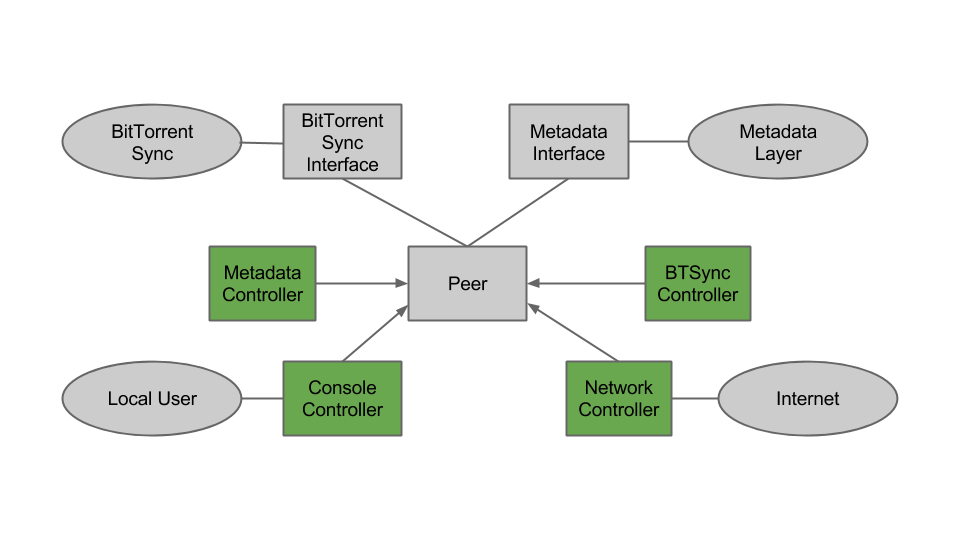
\includegraphics[scale=0.4]{figures/SystemDesign}
  \caption{The design of our system \label{fig:SystemDesign}}
\end{figure}

A high-level overview of our system is offered in Figure \ref{fig:SystemDesign}. We explain each of these components in the following sections.

\subsection{The Data Layer}
% TODO: find out how many unique secret prefixes there are, factoring that into the calculation of how many unique addresses there are.
To implement the data layer of our system, we use BitTorrent Sync. Each peer runs a copy of BitTorrent Sync as a daemon on their system. Our program interacts with it through the use of the BitTorrent Sync API \cite{btsyncapi}, several aspects of which we take advantage of. The first and main aspect is that is takes care of the actual data transfer; so long as our program provides BitTorrent Sync with the appropriate secrets and IP addresses of hosts involved in each file backup, it will take care of all data transfer in the data layer. The second is that the secrets that BitTorrent Sync generates can be used as general-purpose IDs in our system. We use these secrets as IDs for each peer when they join the overlay network, so that peers can be uniquely identified. This is possible due to the massive range of IDs that exist; according to the BitTorrent Sync Technology page, IDs must be at least 20 bytes long \cite{btsynctech}, which gives a minimum address space of $2^{160}$ unique addresses.

There are two downsides to using BitTorrent Sync. The first is that the software is currently closed source. This means that, while BitTorrent claims that BitTorrent Sync is completely secure, we have no know way of confirming this. It also means that we have less control over how our data layer functions and what information can be accessed from it. This is a problem that we had to solve with regard to the challenge mechanism described in Section \ref{subsec:ChallengeMechanism_sec:Fairness_chap:BTBackup}, the solution for which is described in Section \ref{subsubsec:MetadataController_subsec:SystemCore_sec:SystemDesign_chap:Implementation}. Ideally, we would find an open source version of BitTorrent Sync. However, we were not able to find any such systems that were fully functional. The second downside is that BitTorrent Sync is currently in Beta release. This means that, while the system is usable and has all of its features, there still might be many bugs, which leads to more error in our system as a whole.

\subsection{The Metadata Layer} \label{subsec:TheMetadataLayer_sec:SystemDesign}
Due to time constraints, we simplified the implementation of the metadata layer of our system from a DHT to a tracker. As part of this simplification, we ensure that the tracker would not perform noticeably better than a DHT by not making obvious optimizations. To make the future transition to a DHT as easy as possible, we created a standard interface that our program uses to interact with a metadata layer, where each interface call is general enough to be implemented for any type of metadata layer implementation. The following operations are supported:
\begin{description}
\item[Join Network:] The peer registers itself with the overlay network, specifying what ID it wants to use.
\item[Find Closest Node:] Given a valid ID, return the closest ID that is registered in the network. This is used for finding nodes to replicate on. In our implementation this is accomplished via a binary search through the array of all registered keys, giving an average case search time of $O(\log n)$.
\item[Get:] Given an ID, return the Metadata Record of the corresponding node. This is most closely related to the standard get function used in hash tables.
\item[Blacklist Node:] When a peer performs this interface call, it adds its own ID to the list of blacklisters for a specified node.
\item[Backup File:] Register the creation of a newly-created backup with the metadata layer.
\item[Update File Size:] Let the metadata layer know that the size of a given file has changed.
\item[Remove Backup:] Given a file ID and node ID, a peer can remove a specific replica of one of its files.
\end{description}
Our tracker implementation is a standalone multithreaded application. It uses a custom threadpool implementation, called the Dispatcher, to accept several connections at a time from peers to process the interface calls listed above. Each Metadata Record is stored in an unordered map, which maps node IDs to their corresponding record.

\subsection{The Peer}
% abstraction of what the peer is and does (sits below metadata/btsync, sits above system core)
In our implementation, we have a central object called the Peer. The Peer, as the name suggests, is used to represent the information and functionality associated with a single peer in the network. Much of the functionality of the controllers in the system core is implemented as calls to Peer methods. This is because the Peer is what allows access to the data and metadata layers. It also keeps track of the \textit{backed up files} part of the peer's metadata, in a data structure called the LocalBackupInfo. This information is important to all of the controllers in some way, helping to serve as their access to the peer's view of the other parts of the system.

\subsection{System Core}
%Made up of controllers that make the system go
The system core is composed of several controllers, each of which implements a different logical unit of the system. Each controller is explained in detail below.

\subsubsection{Console Controller}
%Takes user input
%the reader can think about this as the ``client'' part of the peer
%Spawns all other controllers
The main purpose of the Console Controller is to allow input to our program from a text console. During runtime, it waits for the user to enter a command, determines which command was entered and with what parameters when applicable, and calls the appropriate function to handle the command. It acts as the main thread of execution in our program. Currently, there are only two commands that are supported via this controller:
\begin{itemize}
\item backup  $<$fileName$>$ - adds a file to backup.
\item rm $<$fileName$>$ - removes a file that is already being backed up.
\end{itemize}
% TODO implement rm command (just send UpdateFileSize(0))

Since the Console Controller runs on the main thread of execution, it manages the life cycle of the other controllers.

\subsubsection{Network Controller} \label{subsubsec:NetworkController_subsec:SystemCore_sec:SystemDesign_chap:Implementation}
%Handles incoming connections from other Peers
%- requests to store data
%- the reader can think of tihs as the ``server'' part of the peer
The Network Controller is used to wait for incoming connections from the network and handle each connection based on the data being sent. It is implemented so that any handler can be registered, making it a flexible solution. We take advantage of this by using it in both our tracker and peer applications. The peer application uses it to handle backup requests from other peers, while the tracker uses it to accept metadata layer requests. If the system is expanded, the Network Controller will have more responsibilities, such as handling DHT requests in the peer and carrying out node challenges.

\subsubsection{BTSync Controller} \label{subsubsec:BTSyncController_subsec:SystemCore_sec:SystemDesign_chap:Implementation}
% think about changing name to something more accurate
%Keeps the metadata layer up to date with local filesize changes of backed up data.
A challenge that is created by having our data layer implemented as a separate application is that the way the two programs view the network needs to be kept in sync. For example, when a file that is tracked by BitTorrent Sync is updated, the changes in content are automatically managed without the intervention of our program. Although BitTorrent Sync will see those changes and update its information accordingly, our program has no way of knowing that a change occurred. To remedy this, we created the BTSync Controller, whose purpose is to periodically query BitTorrent Sync through its API for changes in file size. Each peer stores a local copy of the metadata of its backed up files, which is compared to the data from the API query. If there is any difference in the file sizes, the controller concludes the file size has changed since the last check. In this case, it uses the peer to update the local copy of the metadata and send an update to the metadata layer to register the change in the network.

\subsubsection{Metadata Controller} \label{subsubsec:MetadataController_subsec:SystemCore_sec:SystemDesign_chap:Implementation}
The purpose of the Metadata Controller is similar to that of the BTSync Controller, in the sense that its purpose is to periodically check for changes in the system state. In this case, it is to make sure that sufficient replicas of each file are being maintained.

In our implementation, the Metadata Controller periodically attempts to ping the nodes that are storing data for the peer in order to determine how reliable they are; this is a simplification of the challenge mechanism in Section \ref{subsec:ChallengeMechanism_sec:Fairness_chap:BTBackup}. When a node is deemed consistently unreliable, the Metadata Controller initiates the creation of a new backup and the deletion of the unreliable one.

% TODO talk about specific numbers used to deem unreliability

The Metadata Controller also queries the metadata layer to determine if any peer has stopped backing up to the node it is running on. In this case, it initiates the removal of the stored data.

\chapter{Methodology} \label{chap:Methodology}

In order to thoroughly evaluate our system, we identified several variables that could lead to differences in performance. These variables are:

\begin{itemize}
\item Size of each file being backed up
\item Number of replicas to maintain per file
\item Churn rate
\item Number of nodes present in the system
\item Rate at which nodes are challenged (ping test)
\item Number of malicious nodes
\end{itemize}

From these variables, we derived a set of test scenarios which allowed us to see how each of them affects the performance of the system. While they are specific to our system, they allow us to evaluate the strengths and weaknesses of BitTorrent Sync (and, by extension, BitTorrent) as the data transport mechanism in a peer-to-peer backup system.

The following sections describe how we performed our testing. For the results of each test scenario, see Chapter \ref{chap:Results}.

\section{Environment} \label{sec:Environment_chap:Methodology}

% Ubuntu 12.04 x64 in VM in kvm
% Using SZTAKICloud at MTA SZTAKI in Budapest
% (how much are we allowed to talk about it? ask Mihaly)

% TODO: Is it actually called SZTAKI Cloud? I've looked through my emails, and Mihaly never calls it exactly that.
In order to test our system, we needed an environment that would allow us to create and populate our network with as many nodes as we needed for each test scenario. We used SZTAKI Cloud, a virtualization platform that runs on the enterprise cloud computing system \textit{OpenNebula}. SZTAKI Cloud allowed us to create and clone virtual machines for each test scenario. This is done via its web interface. % TODO: Elaborate more here, depending on how much Mihaly wants us to talk about it.

Each virtual machine was a headless GNU/Linux machine running Ubuntu 12.04, 64-bit. Each machine had a 2.1GB hard drive for the operating system, 1 virtual CPU, and 1GB of RAM. Depending on the test, we also attached another virtual hard drive to each virtual machine, as more storage was needed in order to backup large files.

Each machine is connected to each other via a virtual network that has a 10Gbit link capacity. As this capacity is unrealistic for several of our tests, where the network is supposed to model users spread across the Internet, we used a bandwidth-limiting program called \textit{wondershaper}. \textit{wondershaper} is a command line utility that allows a user to set specific upload and download bandwidth limits on a per-interface basis. This is achieved by creating packet queues. When wondershaper is invoked to limit the bandwidth on a particular interface, it captures all of the packets going through that interface going in either direction. It can then remove them through the queue and send them in the appropriate direction, either towards the network or to a process on the same machine, at a rate specified by the user. The use of this utility allowed us to easily simulate realistic network delays for the tests that needed them.

In order to collect data, we used a logging server, running \textit{syslog-ng}, an open source implementation of the syslog protocol \cite{syslogRFC1,syslogRFC2}. In any syslog implementation, messages are sent and categorized using a facility code, which defines where the message came from and its severity. \cite{syslogRFC1} and \cite{syslogRFC2} specify that there are eight "local use" facilities to be used by processes that have not been assigned a facility. We used one of these for our testing, via the command line \textit{logger} utility that was installed with syslog-ng. All entities that are a part of a test sent log messages to the local use facility. When a test finished, we were able to download the log file and clear it for the next test.

\section{Test Scenarios} \label{sec:TestScenatios_chap:Methodology}

The following sections describes each test scenario, as well as how we performed each test and what variables each scenario tests in particular.

\subsection{File Size versus Number of Files} \label{subsec:FileSizeversusNumberofFiles_sec:TestScenarios_chap:Methodology}

% TODO clarify that we are actually only testing 1 variable here, chunk size
In this scenario, we tested how our system handles a constant amount of data spread out across a varying number of files. We run this test for three reasons. First, it allows us to test the capabilities of BitTorrent Sync in handling a large number of backups. From the data gathered here, it is possible to determine how well BitTorrent Sync would scale for use in a production system, where thousands of users could each be backing up thousands of files of varying sizes. Second, it allows us to measure the performance of BitTorrent against different file sizes. Since the use case for BitTorrent is typically downloading large files, it is important to determine whether or not our system will perform well when users try to backup many small files, should it be used in a production environment. Third, it will demonstrate the ability of our system to backup and recover files faster than if they were transferred by a direct download protocol.

Our tests for this scenario used 8 virtual machines in SZTAKI Cloud: 1 peer, 5 nodes, 1 tracker, and 1 syslog-ng server. To have a wide range of file sizes, we tested with 10MB, 100MB, and 1GB files. In each test instance, the total amount of data backed up was 1GB, so 100 files, 10 files, and 1 file were backed up, respectively. The procedure for each test instance is as follows:

\begin{enumerate}
  \item Clear the log file on the syslog-ng server. This is to remove the data of previous test instances.
  \item Clear all existing items from BitTorrent Sync on the peer and all nodes. This also removes data from previous test instances.
  \item Start the tracker server and all nodes. Both of these entity types do not do anything until the peer joins the network.
  \item Start the peer. When the peer is started, it backs up as many files as the particular instance demands. These backup commands are sent through our program's standard input.
  \item Wait for the peer to find all nodes and create replicas on them.
  \item Stop the nodes and the peer.
  \item Save the log file and reset it.
  \item Restart the nodes.
  \item Remove all backups from the peer. This is done to simulate the peer losing all of its data. The only information that is not removed is a single file generated by our program, which contains all of the information needed to retrieve each backup file.
  \item Start the peer again. The information file is loaded on program startup, which signals BitTorrent Sync to add the backup folders again and contact the appropriate nodes.
  \item Wait for all backups to be restored.
\end{enumerate}

At the end of this sequence, the peer has successfully used our system to backup its files and retrieve them when needed. On the peer and the nodes, the process was orchestrated by a script. Logging occurs during backup creation and retrieval. During both of these phases, the number of bytes being downloaded and uploaded was sampled once per second. This is the data that is sent to the log server. Sampling was achieved by using a series of shell commands to obtain the information and to put it in the useful format. The exact command is as follows:

\begin{verbatim}
sar -n DEV 1 1 | grep eth0 | grep -v Average | \
  awk '{print $1, $2, $6, $7, "\n";}'
\end{verbatim}

The \textit{sar} command retrieves the desired network statistics, from which the other commands extract the specific data we are interested in.

\subsection{Effects of Churn} \label{subsec:EffectsofChurn_sec:TestScenarios_chap:Methodology}

As we have already discussed, churn is important to consider when designing a realistic P2P backup system. The goal of this test scenario is to determine how well our system handles churn. To do this, we created a network of 100 peers, in addition to the tracker and the log server. Each peer had a single 100MB file that it tried to back up. This means that, with five replicas per file, there was 6GB of data in the network, 5GB of which were replica files.
% TODO reword to clarify what "network" means

We measure the effects of churn by logging the number of bytes sent over the network. We gathered this data by using the \textit{ifconfig} command, which reports the total number of bytes that have been sent and received on each interface. For this scenario, we only collected the number of bytes sent by each peer, as the number of bytes received does not take packets lost in the network into consideration. The exact command used is as follows:

\begin{verbatim}
ifconfig eth0 | grep 'TX bytes' | awk -F : '{print $3}' | \
  awk '{print $1}'
\end{verbatim}

where \textit{eth0} is the name of the network interface. With the ability to query this at any time, we were able to determine the number of bytes sent each second by calling the above command once every second. The output is then sent to a logging server, which collects the data from every peer into one log file.

There are two instances within this test scenario. The first is our control, where all peers joined the network at the start and did not leave until the end of the instance. Running this test allowed us to see how much data is transferred without any churn. In the second instance, nodes entered and left the network at a rate specified by a distribution function, described below. By having nodes limit their availability, the peers that store data on them perceive them as unreliable and move their replicas to other nodes, creating more network traffic in the process. By measuring this network traffic and comparing it to the traffic of the test instance with no churn, we can determine the average amount of network traffic generated by data layer maintenance.

% TODO: Make sure this is very understandable.
In our test instance with churn, we modeled a network where each peer had an average uptime of 150 seconds (2.5 minutes) and an average downtime of 75 seconds (1.25 minutes). We chose these numbers based on the amount of time a typical user might be online in a given day. We reasoned that, if a typical user keeps his or her computer on during the day and shuts it off when he or she sleeps (for 8 hours), then the uptime in the average day will be 16 hours. As explained in Section \ref{subsec:ChallengeMechanism_sec:Fairness_chap:BTBackup}, our challenge mechanism sends a challenge message to backup nodes every 6 hours and blacklists them upon 50\% challenge failure over 4 days, meaning that a node is blacklisted if they fail 8 or more challenges. We scaled these numbers down so that we would have a 1 hour test (a factor of 360): a 6 hour challenge becomes a 60 second challenge, and the challenge period becomes 16 minutes. To make the challenge period evenly fit into the 1 hour test, we rounded the challenge period down to 15 minutes, making the scaling a factor of 384. From this factor, we scale 16 hours and 8 hours down to 2.5 minutes and 1.25 minutes, respectively.

To create churn, we have peers enter and leave the network at varying time intervals. The tests were controlled by a Python script that initialized the test environment and ran the test upon machine boot. The script starts and stops BTBackup to simulate the node entering and leaving the network, respectively. To determine the duration of time, the script picked a timeout from one of two distributions, depending on whether the peer was entering or leaving the network.  This is also the strategy used in PeerStore \cite{PeerStore}.

Our distributions are a combination of three functions over the range $[0,1)$. In order to choose an uptime or downtime, a node chooses a random number in this range, and applies it to the following piecewise function:

$$
f(x)=
\begin{cases}
10xc & \mbox{ if $0 \leq x < 0.2$ } \\
[4(x-0.2)+2]c & \mbox{ if $0.2 \leq x < 0.8$ } \\
[e^{21(x-0.8)}+3.4]c & \mbox{ if $0.8 \leq x < 1$ }
\end{cases}
$$

The value of $c$ is what differentiates between choosing an uptime or a downtime. In order to obtain the average uptime and downtime stated above, we used $c=50$ for uptime and $c=25$ for downtime. Since the middle equation is our biggest range, we modeled it so that its average values for each value of $c$ approximately corresponds to the average uptime and downtime. We used a steeper linear equation from 0 to 0.2 so that very short uptimes and downtimes are represented, but very few nodes will ever choose values using this function. The steepness also makes the transition to the middle equation quick but continuous. For the top range, we chose an exponential function so very long uptimes and downtimes are represented. For example, the upper bound for uptime is 3504.32 seconds, or 58.41 minutes for $c=50$, which is almost the entire length of the test. Nodes who pick these values represent computers that are almost always online, such as servers or NAS units.

% TODO cite stats
To make this test scenario more realistic, each node has their upload and download bandwidth limited to different values at the beginning of each instance. Download speeds are picked from a normal distribution of Internet speeds. In order to have a mean and standard deviation for our distribution that is reflective of current Internet speeds around the world, we found statistics on the average download speed per country, as well as the number of people in each country who use the Internet. This allowed us to find the expected value for download speed by taking a weighted average, $W$:
$$
W=\sum\limits_{i=1}^{|\mathcal{D}|} n_iD_i
$$
Where $\mathcal{D}$ is the set of country download speeds and $n$ is the corresponding percentages of global Internet users that each country has. The normal distribution is only used for download speeds; rather than choosing an upload speed using the same method, we took each download speed and divided it by 2.527582524. This ensures that the upload speed is lower than the corresponding download speed, which is often the case on the Internet, as well as ensuring that the two speeds are proportional. We specifically used the aforementioned constant as that was the mean ratio between the two speeds based on the statistics we found.

%By using an exponential distribution, there will be a greater chance of peers going offline for a short amount of time. This is useful, since in a production environment, many nodes will go offline for a short amount of time (i.e. users shutting their machine down at night), but fewer will stay offline for a long period of time or permanently leave the network.

\chapter{Results} \label{chap:Results}

In this chapter, we present the reader with the results of the test scenarios outlined in Section \ref{sec:TestScenatios_chap:Methodology} and their analyses.

\section{File Size versus Number of Files} \label{sec:FileSizeversusNumberofFiles_chap:Results}

In addition to giving us insight into the effects file size and the number of files has on the speed of data backup, we used this test scenario to determine the extent that BitTorrent increases the data transfer rate of file backup and recovery.

\subsection{Data Recovery Speed from Peer's Perspective} \label{subsec:DataRecoverySpeedfromPeersPerspective}

Figure \ref{fig:PeerRecoverySpeed} shows the speed of a peer recovering 1 GB of data in three different situations. Each situation differs in how many files comprise the 1 GB payload: one 1 GB file, ten 100 MB files, and one hundred 10 MB files. The moving average of each data series is shown instead of the raw data to reduce visual clutter; the trends are analogous. The usage of moving averages is the reason why some lines do not cross the x-axis.

\begin{figure}
  \centerline{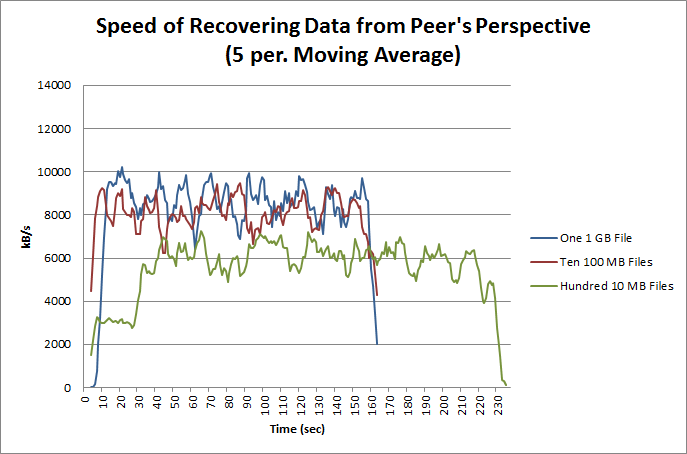
\includegraphics[scale=1]{figures/PeerRecoverySpeed}}
  \caption{The speed at which a peer recovered 1 GB worth of data. \label{fig:PeerRecoverySpeed}}
\end{figure}

It is clear that the peer downloaded its data faster when the data was comprised of fewer files. The peer downloaded the fastest when there was only one file to recover, and the slowest when there were one hundred files to recover. This aligns with the theory behind the BitTorrent protocol, which is designed to transfer larger files quicker.

\begin{table}
\begin{adjustwidth}{-.5in}{-.5in}
\centering
    \begin{tabular}{| l | l | l | l |}
    \hline
    & One 1 GB File & Ten 100 MB files & Hundred 10 MB files \\ \hline
    Mean Speed (kB/s)& 8144.84 & 7874.69 & 5559.32 \\ \hline
    Standard Deviation of Speed (kB/s) & 2564.97 & 1899.86 & 1649.70 \\ \hline
    Median Speed (kB/s)& 9121.41 & 8379.84 & 5874.48 \\ \hline
    Max Speed (kB/s) & 11478.79 & 10948.98 & 8242.56 \\ \hline
    Duration (sec) & 162 & 165 & 231 \\ \hline
    \end{tabular}
    \caption{Statistics on Peer Data Recovery}
    \label{tab:PeerRecoverySpeed}
\end{adjustwidth}
\end{table}

It is worth noting that the increase in speed does not scale linearly with the size of the file. Although the size of the files increased by the same order of magnitude between the trials, the increase in recovery speed seems to have diminishing returns. Table \ref{tab:PeerRecoverySpeed} provides relevant statistics. The mean recovery speed increased by 41.65\% between the "Hundred 10 MB Files" trial and the "Ten 100 MB Files" trial. Compare this to an increase of 3.43\% between the "Ten 100 MB Files" trial and the "One 1 GB File" trial. Looking at it another way, the total time it took to recover the file between the former trials improves by 40\%, whereas the recovery time between the latter trials improves by only 4.76\%.

\subsection{Data Recovery Speed from Nodes' Perspective} \label{subsec:DataRecoverySpeedfromNodesPerspective}

Figure \ref{fig:NodeRecoverySpeed} shows the combined speed at which the nodes are uploading a 1 GB file to a peer during the file recovery process. A moving average is used to reduce visual clutter. We can see a significant improvement between the combined upload speed achieved by all nodes compared to the individual upload speeds of each node.

\begin{figure}
  \centerline{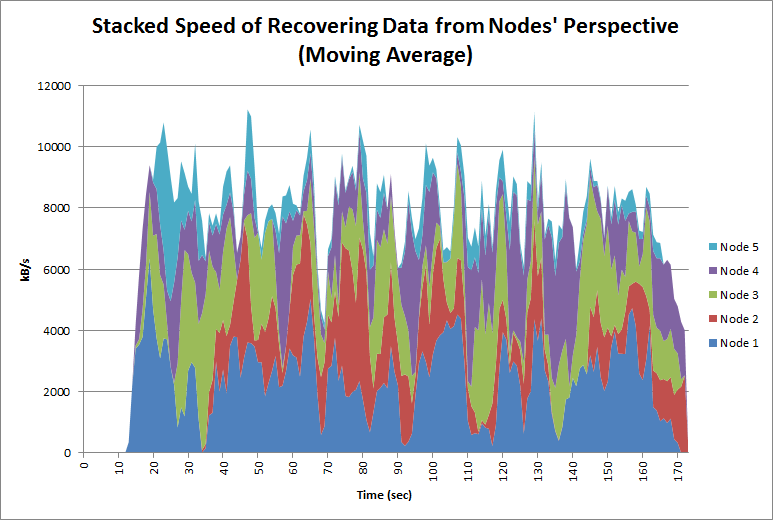
\includegraphics[scale=1]{figures/NodeRecoverySpeed}}
  \caption{The combined speed of nodes uploading a 1 GB file to a peer for file recovery.
  \label{fig:NodeRecoverySpeed}}
\end{figure}

There are a two interesting characteristics of this graph. The first is that data transfer does not start immediately; rather, it starts after the 10 second mark. This happens because the peer must index the file before sending parts of it to each node, as part of the BitTorrent Protocol. The second characteristic is that the data transfer rates for each node vary greatly over time. This can also be attributed to the BitTorrent Protocol: the peer requests file chunks from specific nodes, which corresponds to the peaks in data transfer. With this same reasoning, the peer might not use every node all of the time, which would correspond to the points in the graph where the upload speed drops for specific nodes.

If the peer was restricted to recovering its data from only one node, its download speed would be limited by the node's upload speed. Table \ref{tab:NodeRecoverySpeed} lists the relevant upload speed statistics of the nodes. At best, the peer could download at an average of 2303.07 kB/s. However, by using BitTorrent as a data transfer protocol instead of a direct download, the peer's download speed is limited by the \textit{sum} of each node's upload speed: 7427.61 kB/s. This means, on average, the peer can theoretically download 322.50\% faster!\footnote{This number is based on the mean. The highest median is 2024.57 kB/s and the sum of medians is 4889.01 kB/s, 241.48\% faster.}

\begin{table}
\begin{center}
    \begin{tabular}{| l | l | l | l | l | l |}
    \hline
    & Node 1 & Node 2 & Node 3 & Node 4 & Node 5 \\ \hline
    Mean & 2303.07 & 1293.71 & 1702.47 & 1556.95 & 571.41 \\ \hline
    Standard Deviation & 1921.11 & 1714.13 & 1852.66 & 1796.30 & 1000.72 \\ \hline
    Median & 2024.57 & 477.37 & 1187.60 & 1028.09 & 171.38 \\ \hline
    Max & 7632.07 & 7423.9 & 6936.94 & 7237.46 & 5216.15 \\ \hline
    \end{tabular}
    \caption{Statistics on Node Upload Speed (in kB/s)}
    \label{tab:NodeRecoverySpeed}
\end{center}
\end{table}

\subsection{Entities Backing Up a 1 GB File} \label{subsec:EntitiesBackingUpa1GBFile}

Figure \ref{fig:EntityBackupSpeed} shows the speeds at which each participating entity is backing up a 1 GB file.  We use a 20 period moving average to reduce the visual clutter while keeping the overall trends the same.\footnote{The use of a 20 period moving average significantly alters the peaks and valleys of each line. This is acceptable for our purposes because we are only concerned with each line's existence and relative placement, not its individual details.}

\begin{figure}
  \centerline{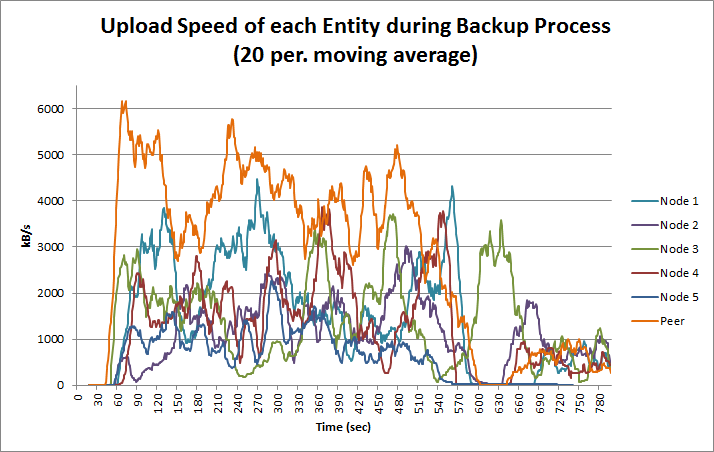
\includegraphics[scale=1]{figures/EntityBackupSpeed}}
  \caption{The speed at which each entity backs up a 1 GB file. \label{fig:EntityBackupSpeed}}
\end{figure}

We confirm that the nodes, in addition to the peer, are actively backing up the peer's file. This is the expected behavior of the BitTorrent protocol, which allows all users in a swarm to share data with each other. BitTorrent Sync, which uses a modified BitTorrent protocol, also seems to leverage this feature.

The peer generally uploads the fastest for the first 9 minutes; the nodes are all requesting chunks from mostly the peer throughout this period, as it is the initial seeder. However, around the 9 minute mark, the nodes seem to start requesting data from each other more often than the peer, as seen by the peer's decrease in upload speed between the 9 and 10 minute mark. Another interesting phenomenon occurs directly after this interval, from 11 minutes onward: the upload speed for most of the nodes picks up again, while the peer's upload speed drops to a similar rate. While it is difficult to determine exactly why this happens, since we do not have access to the exact version of the BitTorrent protocol that BitTorrent Sync uses, we theorize that this change is a reflection of BitTorrent distributing the work of uploading to the nodes. At the end of our tests, we noticed that all nodes had almost the entire file downloaded, with the exception of one, which had almost half the file left to download. It is possible that when nodes are close to being finished with the download, they work together to help other nodes get to a similar state. In this case, four of the nodes and the peer would be uploading to the fifth node, whose upload speeds looks like it is 0kB/s from around 9 minutes onward.

As with \ref{fig:NodeRecoverySpeed}, we believe the interval of time at the start of the test with no activity is due to BitTorrent Sync indexing the 1 GB file before it can transfer it.

% TODO rename this test to 'Data Backup Speed From Peer's Perspective' or something, discuss increase in backup speeds (upload speed of peer vs upload speed of peer + upload speed of nodes. need to do algebra to figure out speed increase)

\section{Effects of Churn} \label{sec:EffectsofChurn}

This scenario was comprised of 100 peers each replicating a 100mb file 5 times, meaning there was theoretically a total of 50 GB of data in the network, ignoring the effects of churn. Table \ref{tab:ChurnBandwidth} summarizes the actual amount of data in the network, with and without churn.

\begin{table}
\begin{center}
    \begin{tabular}{| l | l |}
    \hline
    Without Churn & With Churn \\ \hline
    58.00 GB & 72.27 GB\\ \hline
    \end{tabular}
    \caption{Amount of data transferred in a 100 node network over 1 hour}
    \label{tab:ChurnBandwidth}
\end{center}
\end{table}

First, notice that the actual amount of data sent in the network without churn was 58 GB, 8 GB more than the calculated theoretical value. Distributed over 100 machines, this means each peer sent an additional 80 MB of data on average into the network throughout the duration of the test. Extra network traffic produced by our system could have contributed to this discrepancy, including communications with the tracker and each other. BitTorrent Sync could also be responsible, since there is overhead associated with both the metadata it maintains to stay synchronized, and the BitTorrent protocol it uses (e.g., requesting chunks of data from ). Communications between the script that instrumented the test and the log server may also have generated a nontrivial amount of traffic.

We designed this scenario to simulate an average level of churn over 16 days. The difference in data sent between the instance with churn and the one without is 14.27 GB. This means, on average, each peer sent an additional 142.7 MB of data in the presence of churn. In other words, with our system, the average peer can expect to create an additional replica every $\dfrac{16 \text{ days}}{142.7 \text{ MB}} \times 100 \text{ MB per replica} = 11.21 \text{ days}$.

It is important to note that this number is specific to the conditions that we have created for this test scenario. It is possible that a greater or lesser amount of churn would be present in a production environment; the amount that we have chosen is an approximation. The users of our system would be the ones to determine the availability of the average peer in the network. For example, if many users have servers, NAS devices, or other machines that are constantly online and are contributing resources to the network, the amount of churn will be lower, and therefore less replicas will need to be moved on average. The network could also be mainly made up of users who keep their computers off for most of the day, in which case the amount of traffic generated would be much higher. Since we have modeled our churn rate off of the average user, the results of our tests should be reflective of what would be seen in a production system.

\section{Summary}

% TODO - do we actually test this now that we aren't doing the 1000x1mb test? may need to remove goal from methodology.
% 1. how well does btsync handle large number backups? how well will it scale?

Section \ref{subsec:DataRecoverySpeedfromPeersPerspective} compared how our system performs when recovering many small files versus few large files. We concluded that there is a large performance gain by recovering fewer, larger files, but the returns diminish between files of size 100 MB and 1 GB.

Section \ref{subsec:DataRecoverySpeedfromNodesPerspective} verified our hypothesis that our system would recover data faster than an equivalent one using a direct download data transfer protocol. Our data suggests that the speed increase could be upwards of 300\%. This is possible, because the use of multiple nodes in a file recovery allows the download bandwidth of the peer to be fully utilized.

Section \ref{subsec:EntitiesBackingUpa1GBFile} showed that our system lessens the Peer's load of backing up a file by distributing the task to the nodes as well. This has the side effect of speeding up the backup process, because nodes upload the data they have at a given time to each other, better utilizing their download bandwidth. It is important to consider the number of replicas per file here, because the replica count that is maintained affects the speed and bandwidth usage of the backup and restore procedures. As the number of replicas per file increases, more traffic must be generated to create and maintain those replicas, but the download speed when recovering will be greatly improved. Of course, the maximum recovery speed is limited by the peer's download bandwidth.

Section \ref{sec:EffectsofChurn} explained that, in the presence of an average amount of churn, the average peer would need to make a new replica of any given file every 11 days. This time interval is derived by taking the average amount of time between the creation of replicas in our test instance and scaling that number based on the scaling factor that we used for the entire test instance.

\chapter{Conclusion} \label{chap:Conclusion}

As consumer technology improves and higher resolution content can be generated and used by more people, the need for higher capacity backup systems increases. Most backup systems that have gained popularity have a centralized model, where backups are created on the storage servers of the entity that is offering the service. While this system model is practical for backing up a small amount of data, it is not a suitable option for users who need to backup a large amount of data, because these services often come with a data cap. Additional space is only obtainable by paying a fee.

The alternative to centralized backup systems are Peer-to-Peer systems, where peers use each other as storage sites for their backups. By distributing the storage available to the network in this way, there is no central entity that the users need to rely on. In addition, the amount of storage space scales with the size of the network, since all users must offer space if they want to use the space of others. This means that, instead of paying for remote storage space in money, users "pay" for the storage with their own storage space.

There are several challenges to creating a robust and reliability P2P backup system, however. Without the existence of a central entity that is solely dedicated to storing the files of others, it is possible that one's backups could be inaccessible at any given time, since regular users will often shut their computers off. Keeping track of who stores what data and making sure that everyone is contributing fairly are also major concerns. In addition to these problems, P2P backup systems share another problem with centralized systems: if users want to backup large amounts of data, the process of transferring these data is lengthy and inconvenient.

To address these problems, we have proposed a new P2P file backup system, which we call BTBackup. BTBackup uses concepts from existing research on P2P backup systems to address most of the problems stated above. However, the main focus of BTBackup is to address to problem of slow backup creation and restoration. This was accomplished via the use of BitTorrent Sync, which uses the BitTorrent protocol to transfer data. By using this protocol, peers can maximize their use of both upload and download bandwidth when creating backups and restoring files.

To test whether or not our system provided an increase in file transfer speeds, in addition to providing solutions for the other challenges of P2P backup systems, we implemented a prototype of our system and tested it on a virtualized, 100 node network using MTA SZTAKI's cloud computing system. We found that it was able to handle node churn with a reasonable amount of overhead in network traffic, requiring the replacement of a replica every 11 days. More importantly, however, we found that our system allowed for a \~300\% improvement in file restoration speeds. This would not be possible if these data transfers were only between a user and some other entity, whether it is the service provider in a centralized backup system or a single peer in another P2P backup system.
% TODO add (first, create) result of file backup increase

\section{Future Work}

\subsection{BTBackup Security} \label{subsec:BTBackupSecurity}

We would like to see our system design incorporate security. Specifically, the DHT should have some scheme that ensures (1) entries cannot be tampered with by the node responsible for them and (2) nodes cannot lie about the data with which they are involved. We believe both of these goals can be achieved through the use of chained digital signatures.

Regarding (1), there could be a digital signature encompassing the entire entry to prevent the responsible node from modifying it. Perhaps the node that the entry describes could digitally sign it upon modification; or maybe the most recent node to modify an entry could digitally sign it. These solutions solve the immediate problem, but bring about additional ones that need to be investigated.

An example solution for (2): the communication between peers during the "Finding Replication Nodes" phase of backing up a file could be extended to require both parties digitally sign the information. That is, when a peer informs a node it will be backing up a given file of a given size, the DHT can store an additional entry containing their digital signatures, binding them to the exchange. This provides non-repudiation for the amount of data a peer is backing up and a node is storing, each of which a malicious user is incentivized to lie about. This solution does not deal with the blacklisters data, though a similar scheme for that is easy to imagine.

To reduce the size of the DHT with the addition of these digital signatures, a chaining mechanism could be put in place, similar to the one in Bitcoin's blockchain. Instead of appending digital signatures to the corresponding DHT column, new digital signatures could sign the old ones and then overwrite them. This preserves their effect, but removes the associated storage cost. More thought needs to be given to this to design an optimal mechanism (and to determine if chaining is even required).


\subsection{NAT Traversal}

We have designed our system so that peers directly contact each other by their IP address. While there are no problems with this solution when all peers are directly visible to the public Internet, it does pose a problem when they are behind a router that uses Network Address Translation, or NAT. When one or more hosts are behind a NAT-enabled router, they send network packets that have a destination outside of their subnet to the router. The router creates mappings between the hosts' internal IP address and the ports that they are using to the router's publicly visible IP address and a port that is chosen by the router. This is convenient for the typical home user, since Internet Service Providers typically only give one public IP address per Internet subscription. A home user can connect multiple devices to the NAT-enabled router, and they will all seem to be one device (with the router's public IP address) to the rest of the Internet. While it is convenient, it comes at the cost of not being able to initiate a connection to a device behind a NAT, since no IP/port mapping has been made yet. This is the case with most home users today, so we would need to design some mechanism to overcome this in our system if it were to be used by people all over the world. We can turn to Skype, BitTorrent, BitTorrent Sync, and other P2P applications for inspiration. These applications and protocols use mechanisms such as publicly visible supernodes as relay servers \cite{skypeSupernode}, trackers \cite{bittorrentProtocol}, and Universal Plug and Play (UPnP) \cite{btsynctech}.

\subsection{Finding the optimal number of replications}

In order to minimize storage overhead, we would like to find the optimal number of data replicas to create before their provided speed enhancement is outweighed by their storage cost.

Our approach takes advantage of the need for replicas in a P2P backup system to combat node churn; we use the already-present replication nodes as a BitTorrent swarm, which provides the speed boost without additional overhead. However, we wonder if the cost of creating replicas in addition to the ones needed for data availability would improve the data transfer rate even more. The fact that the additional replicas also provide greater data availability should also be taken into account.

Optimally, we would want to determine the minimum number of replicas needed in order to provide data availability while still taking advantage of the speed boost provided by BitTorrent. In order to determine this number, further tests could be done on our system that modifies the number of replicas that a peer seeks to create. The download and uploads speeds would then be measured for each replica count and compared to each other in order to determine if there are any differences. In order to also test data availability, the tests could factor in a rate of churn, similar to the test scenario described in section \ref{subsec:EffectsofChurn_sec:TestScenarios_chap:Methodology}. The availability of replicas would then be measured based on our system's challenge mechanism.

\subsection{BTBackup Implementation}

There are many features missing from our implementation that we would like to see added. A brief, nonexhaustive list follows. It does not include other future work detailed in this chapter.

\begin{itemize}
    \item Replace the centralized tracker with a DHT to become completely decentralized.
    \item Encrypted communication between peers to reduce information leakage.\footnote{The actual transfer of data is already encrypted; this item refers to the transfer of encryption secrets and challenge messages.}
    \item The ability to backup folders, not just files.
    \item Implement a more sophisticated challenge mechanism. Our current implementation of the challenge mechanism only checks for node availability. In order to have a system where all peers are storing the amount of data they are supposed to, the challenge mechanism we described in section \ref{subsec:ChallengeMechanism_sec:Fairness_chap:BTBackup} will need to be implemented.
    \item Use only open source software. Currently, BitTorrent Sync is closed source. In order to ensure that the system can be completely trusted, we would either need to wait for BitTorrent Sync to become open source, use an open source alternative, or create our own.
\end{itemize}

% TODO reformat some citations to include volume number, etc
\begin{thebibliography}{11}

\bibitem{dropboxusers} https://www.dropbox.com/news/company-info
\bibitem{oneddriveusers} http://blog.onedrive.com/over-250m-people-using-skydrive/
    
\bibitem{ChurnResilient} S. Legtchenko, S. Monnet, P. Sens, G. Muller, Churn-Resilient Replication Strategy for Peer-to-Peer Distributed Hash-Tables
\bibitem{Kademlia} P. Maymounkov, D. Mazi\`eres, Kademlia: A Peer-to-Peer Information System Based on the XOR Metric

\bibitem{pStore} C. Batten, K. Barr, A. Saraf, S. Trepetin, pStore: A Secure Peer-to-Peer Backup System
\bibitem{PeerStore} M. Landers, H. Zhang, K. Tan, PeerStore: Better Performance by Relaxing in Peer-to-Peer Backup
\bibitem{StorageSearchP2PNetworks} J. Augustine, A. Molla, E. Morsy, G. Pandurangan, Storage and Search in Dynamic Peer-to-Peer Networks
\bibitem{p2pSurvey} A. Passarella, A survey on content-centric technologies for the current Internet: CDN and P2P solutions

\bibitem{BTSyncFAQ} http://www.bittorrent.com/help/faq/sync
\bibitem{btsynctech} http://www.bittorrent.com/sync/technology
\bibitem{btsyncuserguide} http://btsync.s3-website-us-east-1.amazonaws.com/BitTorrentSyncUserGuide.pdf
\bibitem{btsyncapi} http://www.bittorrent.com/sync/developers/api

\bibitem{cryptoDef} Rivest, Ronald L. (1990). "Cryptology". In J. Van Leeuwen. Handbook of Theoretical Computer Science 1. Elsevier.
\bibitem{bittorrentDHT} http://www.bittorrent.org/beps/bep\_0005.html
\bibitem{bittorrentProtocol} http://www.bittorrent.org/beps/bep\_0003.html
\bibitem{syslogRFC1} C. Lonvick, "The BSD syslog Protocol". https://tools.ietf.org/html/rfc3164, August 2001.
\bibitem{syslogRFC2} R. Gerhards, "The syslog Protocol". https://tools.ietf.org/html/rfc5424, March 2009.
\bibitem{skypeSupernode} S. Guha, N. Daswani, R. Jain, "An Experimental Study of the Skype Peer-to-Peer VoIP System". http://saikat.guha.cc/pub/iptps06-skype/ .

\end{thebibliography}

\end{document} 